



%----------------------------------------------------------------------------------------

\newpage

%%%%%%%%%%%%%%%%%%%%%%%
\section{Network growth heuristics}{Heuristiques de génération de réseau}

\label{app:sec:networkgrowth}

Les espaces topologiques des réseaux générés en~\ref{sec:networkgrowth} peuvent être conditionnés aux classes morphologiques pour la distribution de densité initiale. Ce conditionnement est montré en Fig.~\ref{fig:app:networkgrowth:feasiblespace_bymorph}


%%%%%%%%%%%%%%%%%
\begin{figure}
%\includegraphics[width=\linewidth]{Figures/NetworkGrowth/feasible_space_pca_bymorph}
%\includegraphics[width=\linewidth]{Figures/NetworkGrowth/feasible_space_withreal_pca_bymorph}
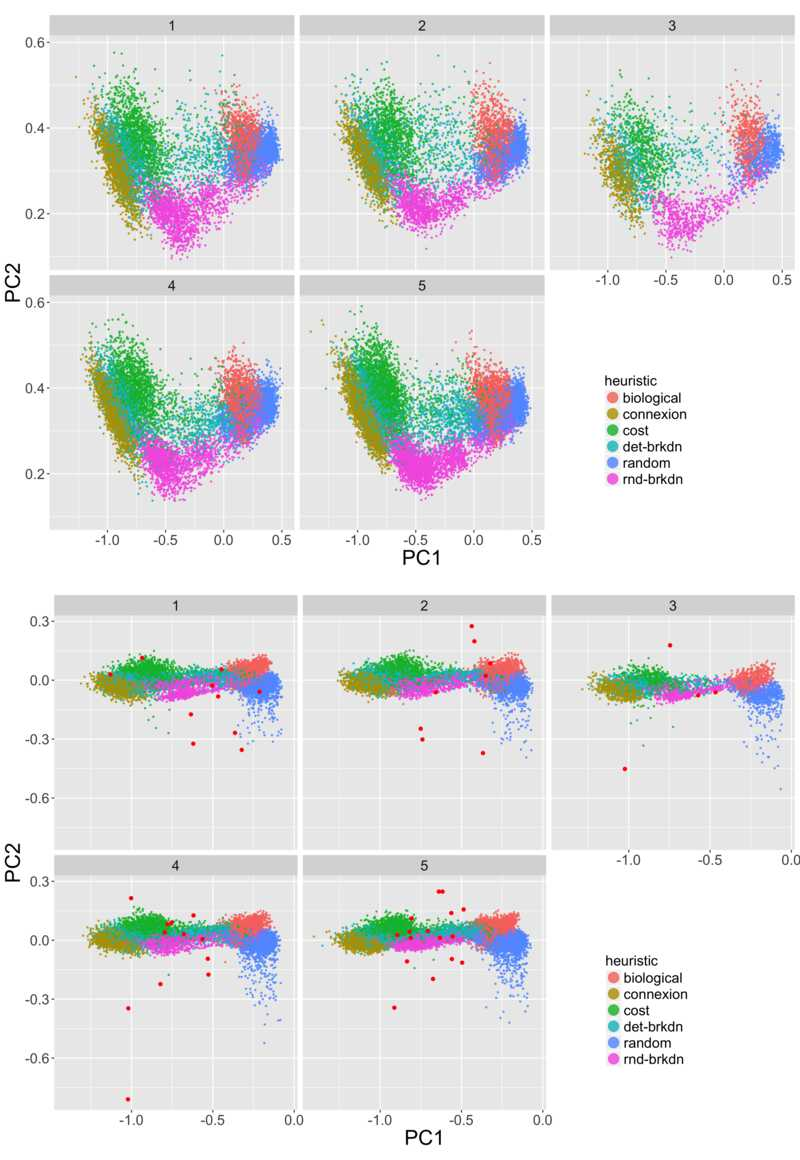
\includegraphics[width=0.9\linewidth]{Figures/Final/A-networkgrowth-feasiblespace_bymorph}
\appcaption{}{\textbf{Espace topologique faisable pour les différentes heuristiques de génération, conditionné à la classe morphologique de densité.}\label{fig:app:networkgrowth:feasiblespace_bymorph}}
\end{figure}
%%%%%%%%%%%%%%%%%














%----------------------------------------------------------------------------------------

\newpage

%%%%%%%%%%%%%%%%%%%%%%%
\section{Transportation Network Governance modeling}{Modélisation de la gouvernance du système de transport}

\label{app:sec:lutecia}


%%%%%%%%%%%%%%%%%%%%%%%
\subsection{Semi-analytical study of the land-use model}{Modèle d'usage du sol}


\subsubsection{Convergence}{Convergence}

Nous étudions ici la question de la convergence dans le temps de la distribution des activités, à infrastructure fixe.

Considérons un cas très simple : en prenant $\lambda = 0$ on déspatialise le problème et en prenant $\gamma_A = 1$ on finit de découpler population et emplois. En posant $\beta' = \sum_j E_j \cdot \beta$ et $P_0 = \alpha \cdot \sum_i P_i$, l'existence d'un point fixe pour les populations se ramène à la résolution de
\[
P_i = P_0 \cdot \frac{\exp\left(\beta' \cdot P_i\right)}{\sum \exp\left(\beta' \cdot P_i\right)}
\]

La fonction est bien continue en les $P_i$ et les plages de variations de la population sont $[0,\sum_i P_i]$, elle admet donc un point fixe par le Théorème du Point Fixe de Brouwer. 

En fait, en toute généralité, si on écrit

\[
(\vec{P}(t+1),\vec{E}(t+1)) = f(\vec{P}(t),\vec{E}(t))
\]

pour des valeurs des paramètres arbitraires, la fonction $f$ est également continue en chaque composante, et prend ses valeurs dans un fermé borné (les emplois étant également limités) donc compact. De la même manière que \cite{leurent2014user} l'établit pour un modèle de flux de traffic, on a aussi un point fixe dans notre cas, ce qui correspond à un point d'équilibre. L'unicité n'est cependant pas triviale et il n'y a pas de raison qu'elle soit vérifiée a priori. On vérifie empiriquement la convergence systématique à infrastructure fixe (voir ci-dessous l'exploration de l'espace des paramètres).


\subsubsection{Exploration}{Exploration}


Nous procédons à une exploration du comportement du modèle d'usage du sol seul, i.e. à infrastructure fixe, afin de comprendre l'influence des paramètres sur la forme urbaine. Nous fixons $\alpha = 1$ ici pour étudier le modèle dans un cas extrême.

Nous suivons les indicateurs de forme urbaine définis en~\ref{sec:staticcorrelations}, pour la distribution de la population et pour les emplois, dans le temps et jusqu'après convergence. Nous réduisons l'espace morphologique de la distribution spatiale des actifs dans un plan principal, tel que $PC_1 = -0.98 \cdot I - 0.13 \cdot \mathcal{E} + 0.05 \bar{d} - 0.13 \cdot \gamma $ et $PC_2 = -0.19 \cdot I + 0.57 \cdot \mathcal{E} - 0.16 \bar{d} + 0.77 \cdot \gamma $. La première composante exprime un niveau de dispersion et la seconde une agrégation hiérarchique.


La Fig.~\ref{fig:app:lutecia:morphotrajs} donne des trajectoires temporelles dans le plan $(PC_1,PC_2)$ pour $\gamma_A = 0.9$, $\gamma_E = 0.6$, $v_0 = 6$, pour différentes valeurs de $\lambda$ et de $\beta$ ainsi que pour différents réseaux initiaux.

% morphoActiveTrajs_gammaCDA0.9_gammaCDE0.6
% Morphology
% "PC1" "PC2" "PC3" "PC4"
%"moranActives" -0.980084779269111 -0.195512301926648 -0.0273364571430177 0.0214821635602741
%"entropyActives" -0.137030712105593 0.570339690854727 0.221651600681317 -0.778977399473809
%"meanDistanceActives" 0.0503574253429071 -0.168869841317757 -0.903924010571035 -0.389703078662877
%"slopeActives" -0.134612551783578 0.779724665202014 -0.364752887773974 0.490779215369261



%%%%%%%%%%%%%%
\begin{figure}
	%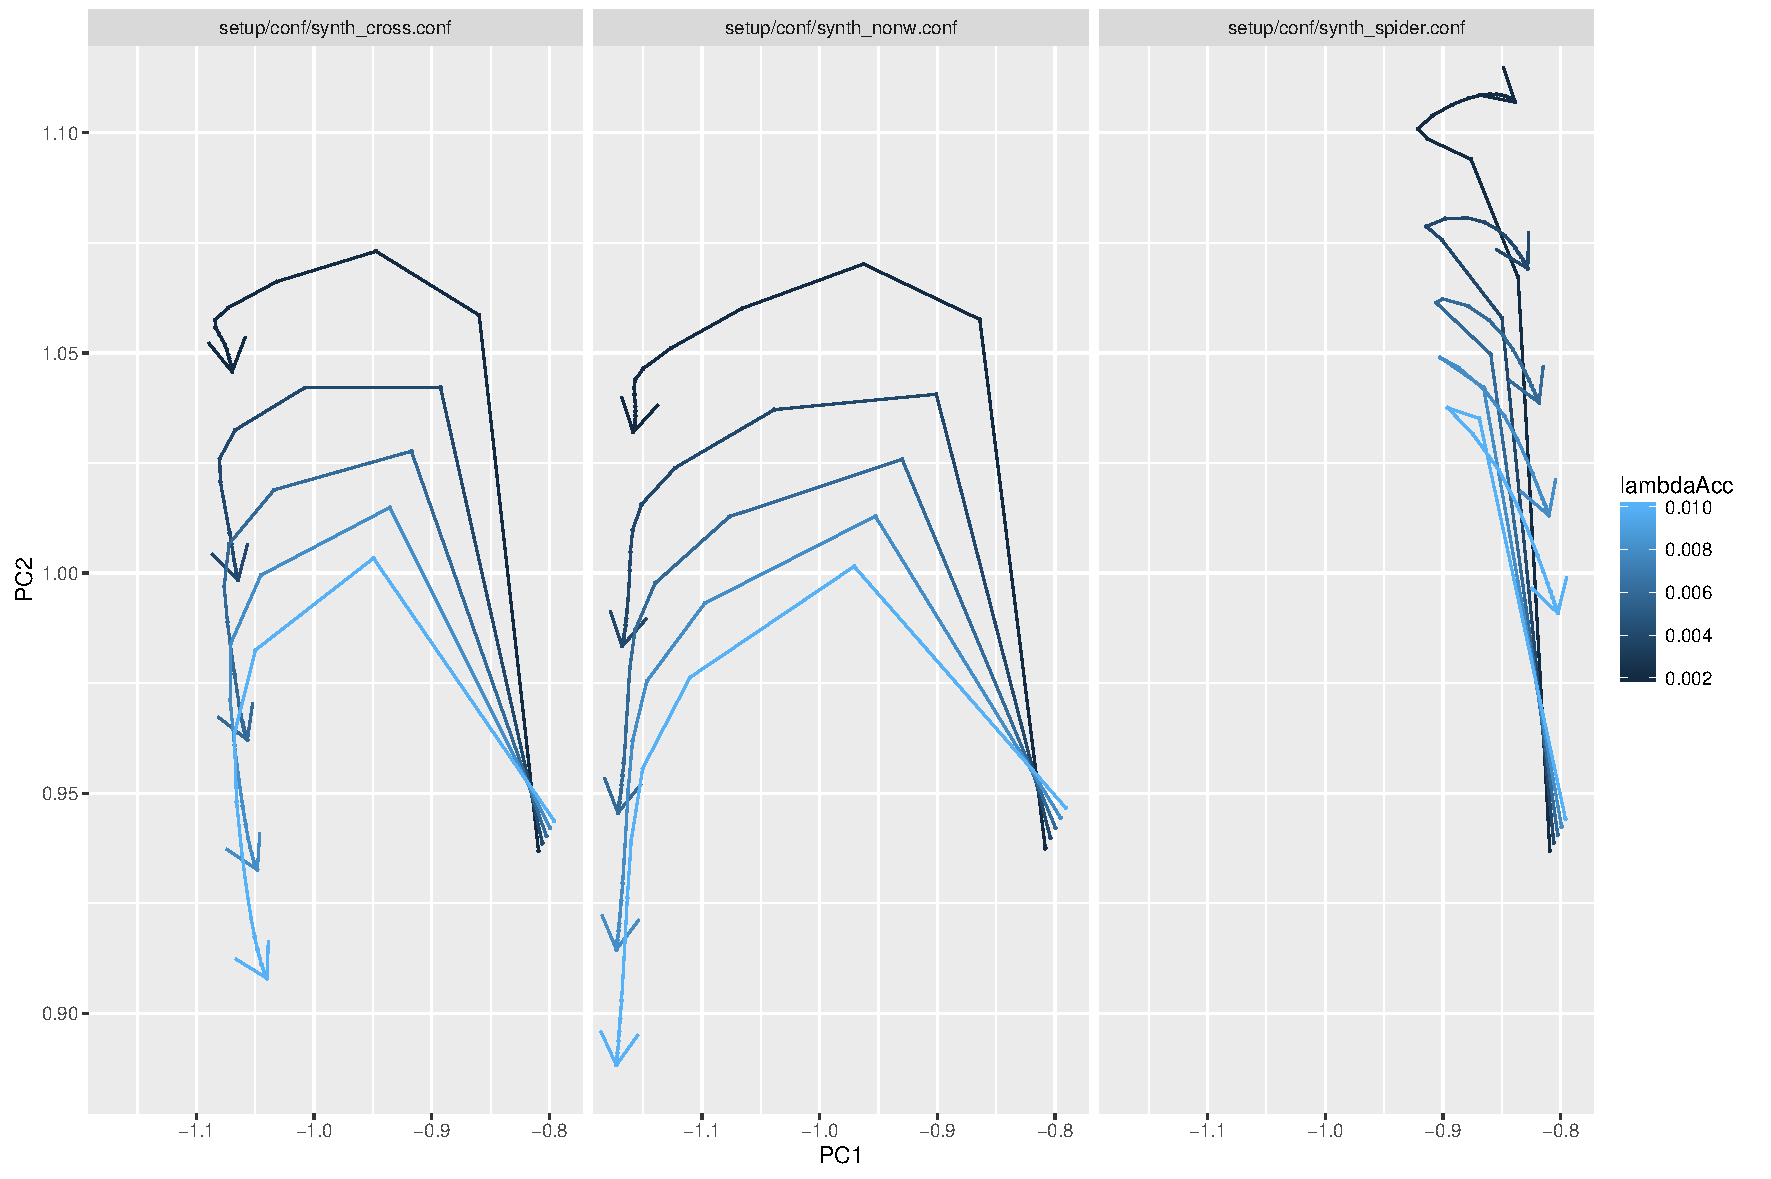
\includegraphics[width=\linewidth]{Figures/Lutecia/morphoActiveTrajsvaryinglambda_betaDC1_euclpace6.pdf}
	%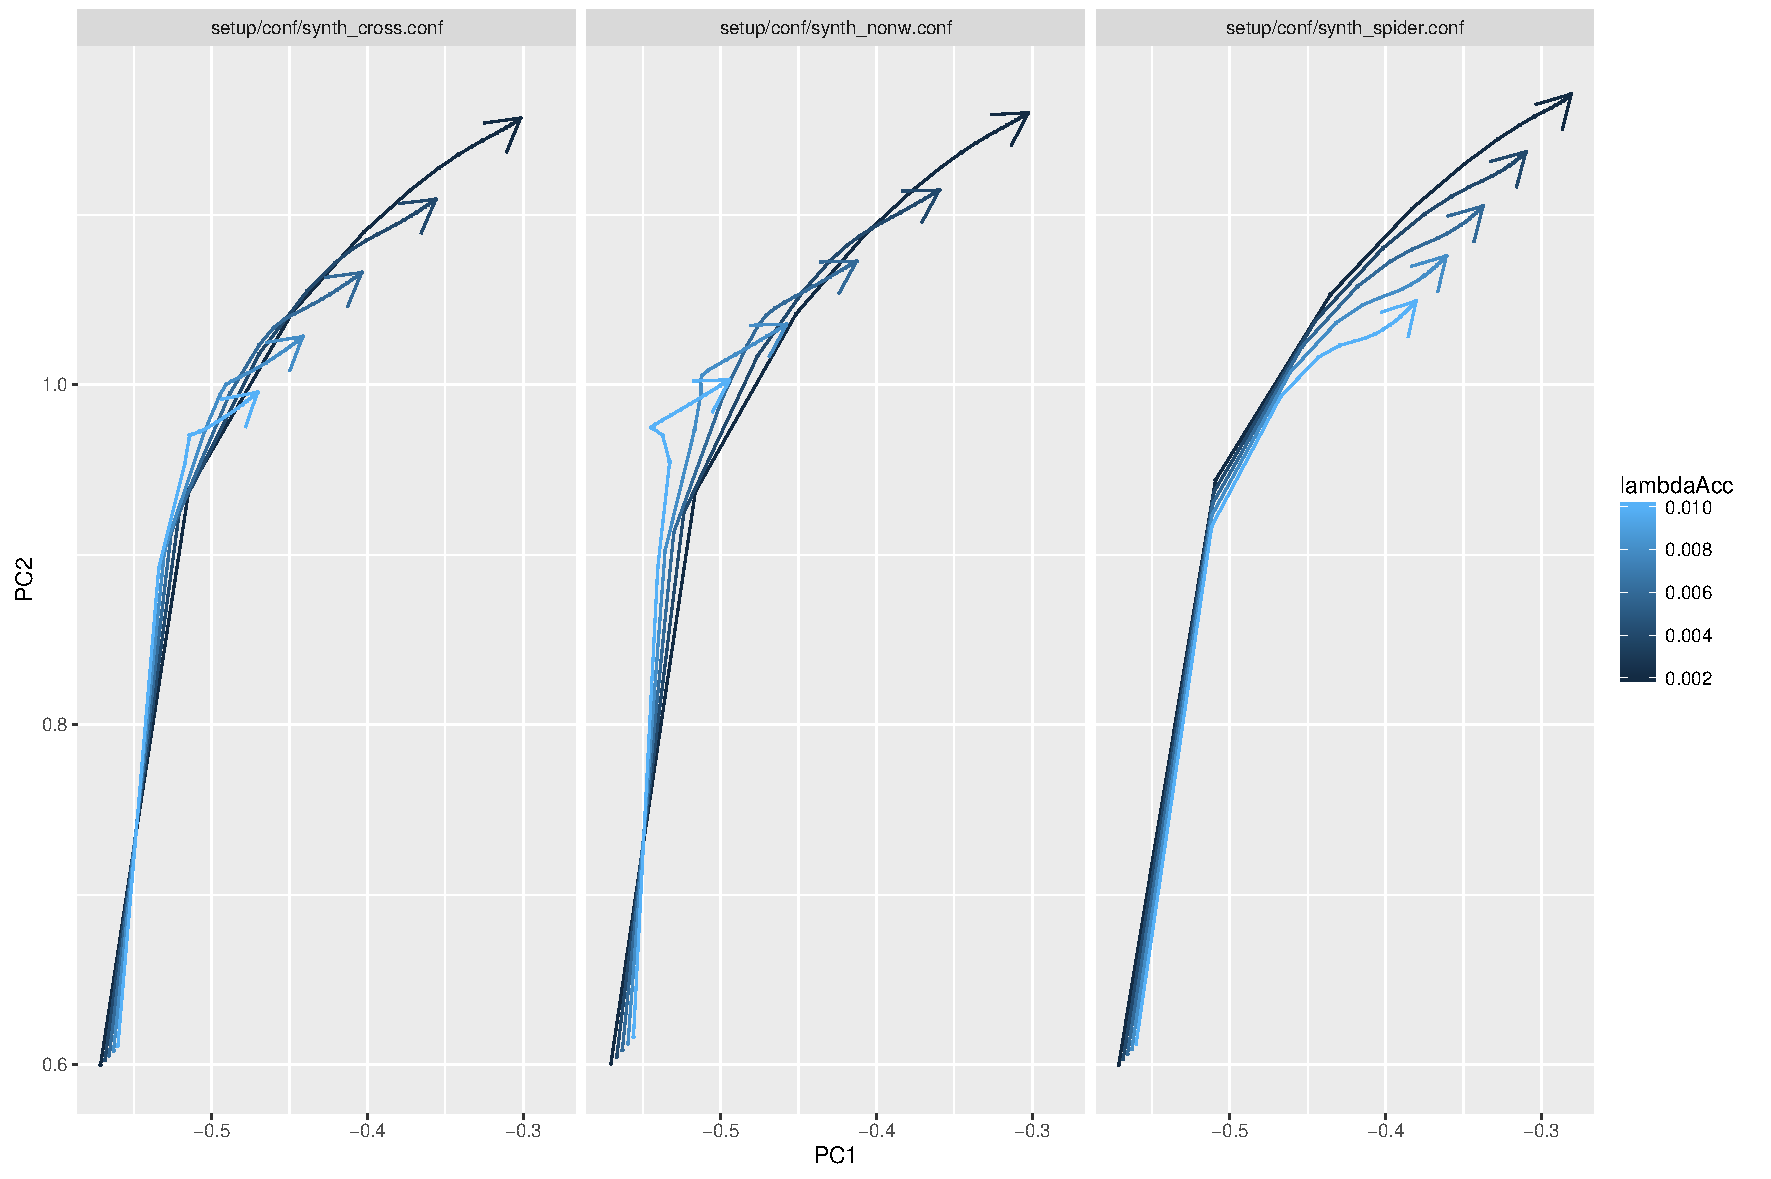
\includegraphics[width=\linewidth]{Figures/Lutecia/morphoActiveTrajsvaryinglambda_betaDC2_euclpace6.pdf}
	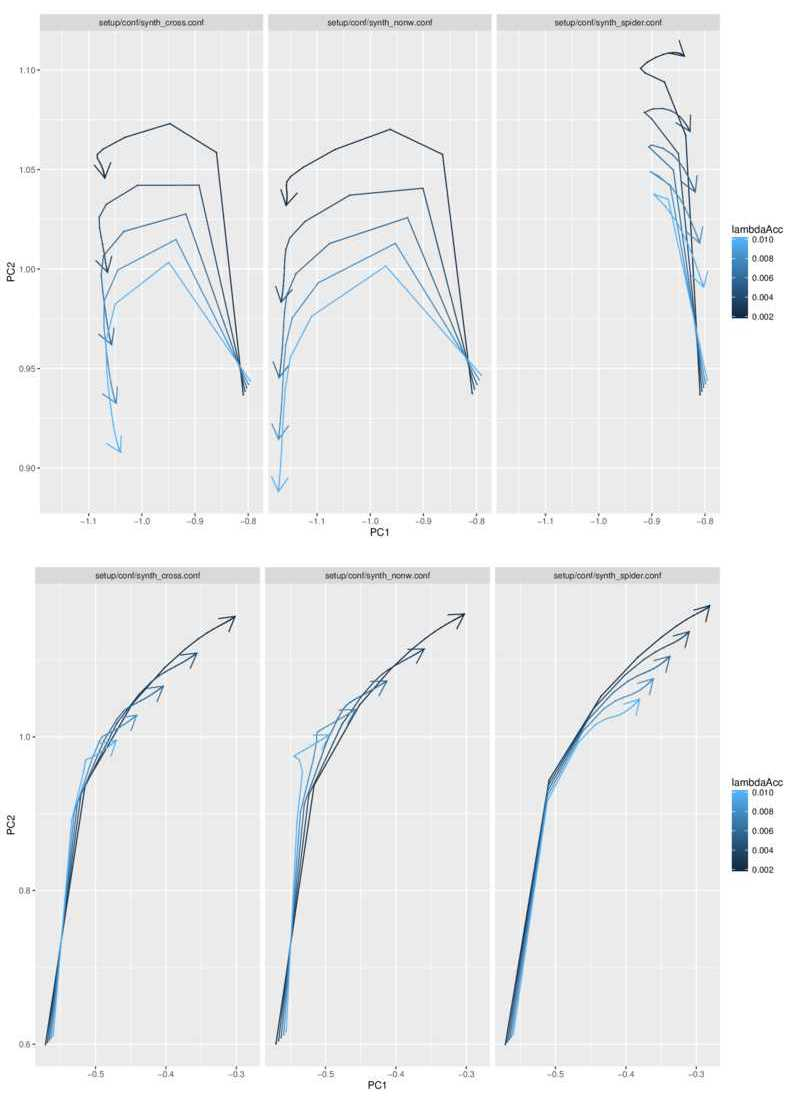
\includegraphics[width=\linewidth]{Figures/Final/A-lutecia-morphotrajs.jpg}
	\appcaption{\label{fig:app:lutecia:morphotrajs}}{\textbf{Trajectoires morphologiques}\label{fig:app:lutecia:morphotrajs}}
\end{figure}
%%%%%%%%%%%%%%


La Fig.~\ref{fig:app:lutecia:morphosens} donne la valeur de $PC_1$ sur l'ensemble de l'espace des paramètres exploré.


%%%%%%%%%%%%%%
\begin{figure}
	%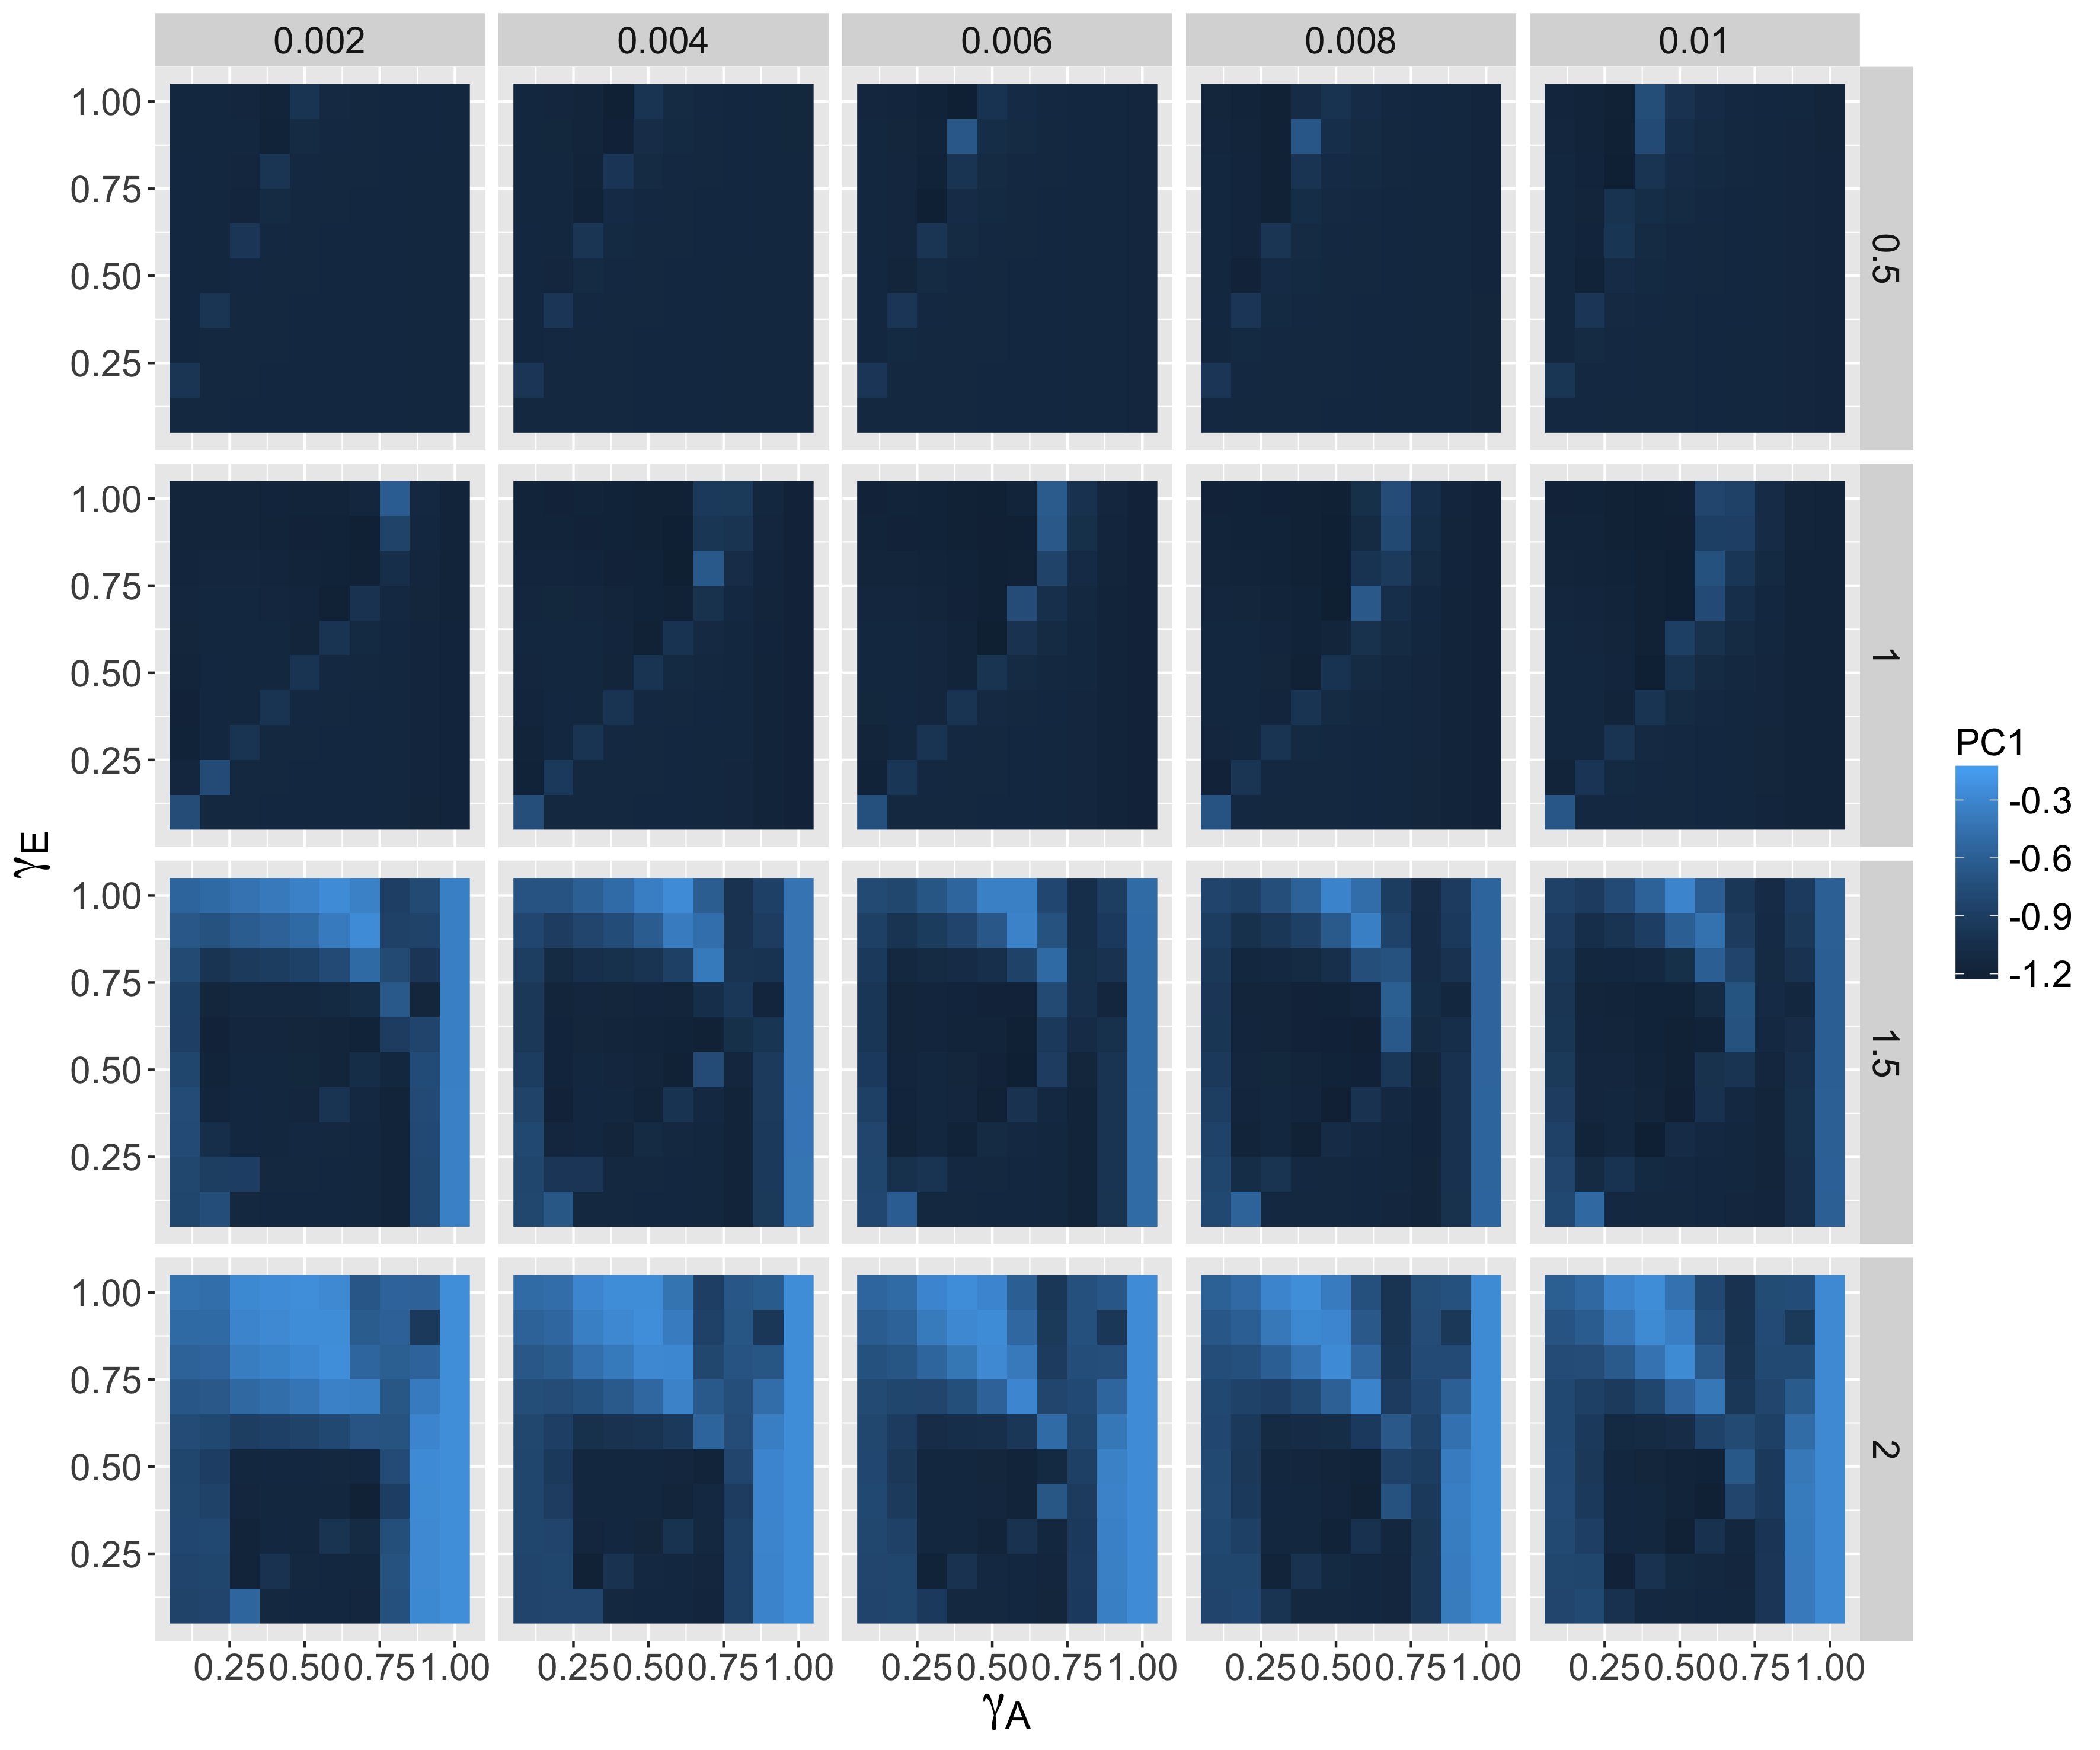
\includegraphics[width=\linewidth]{Figures/Lutecia/PC1_synth_nonw_euclpace6.png}
	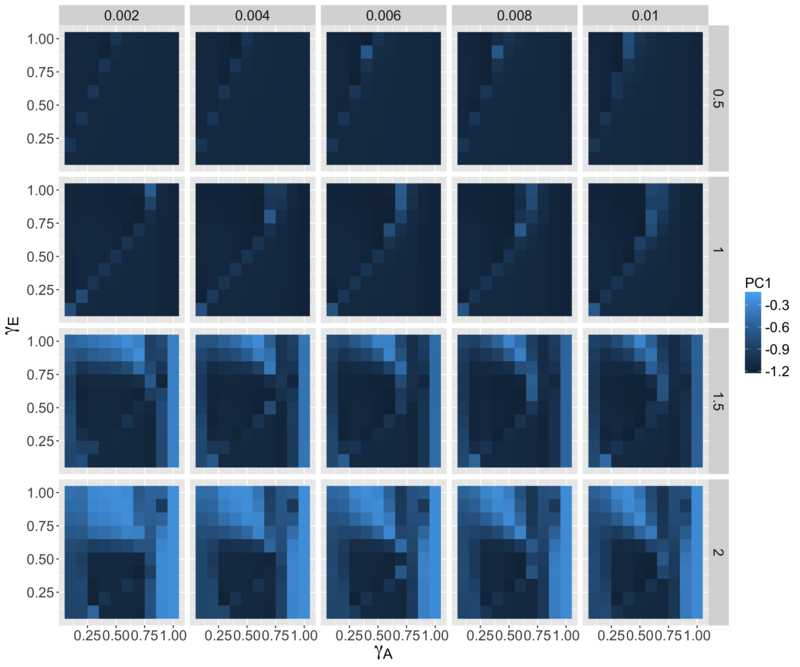
\includegraphics[width=\linewidth]{Figures/Final/A-lutecia-morphosens.jpg}
	\appcaption{\textbf{Sensitivity of the urban form.}\label{fig:app:lutecia:morphosens}}{\textbf{Sensibilité de la forme urbaine.}\label{fig:app:lutecia:morphosens}}
\end{figure}
%%%%%%%%%%%%%%



Enfin, afin de comprendre l'influence des paramètres sur la mobilité totale au cours d'une trajectoire complète, nous étudions en Fig.~\ref{fig:app:lutecia:ludiff} la variation cumulée donnée par $\sum_t \sum_k \left|\Delta A_k (t)\right|$.


%%%%%%%%%%%%%%
\begin{figure}
	%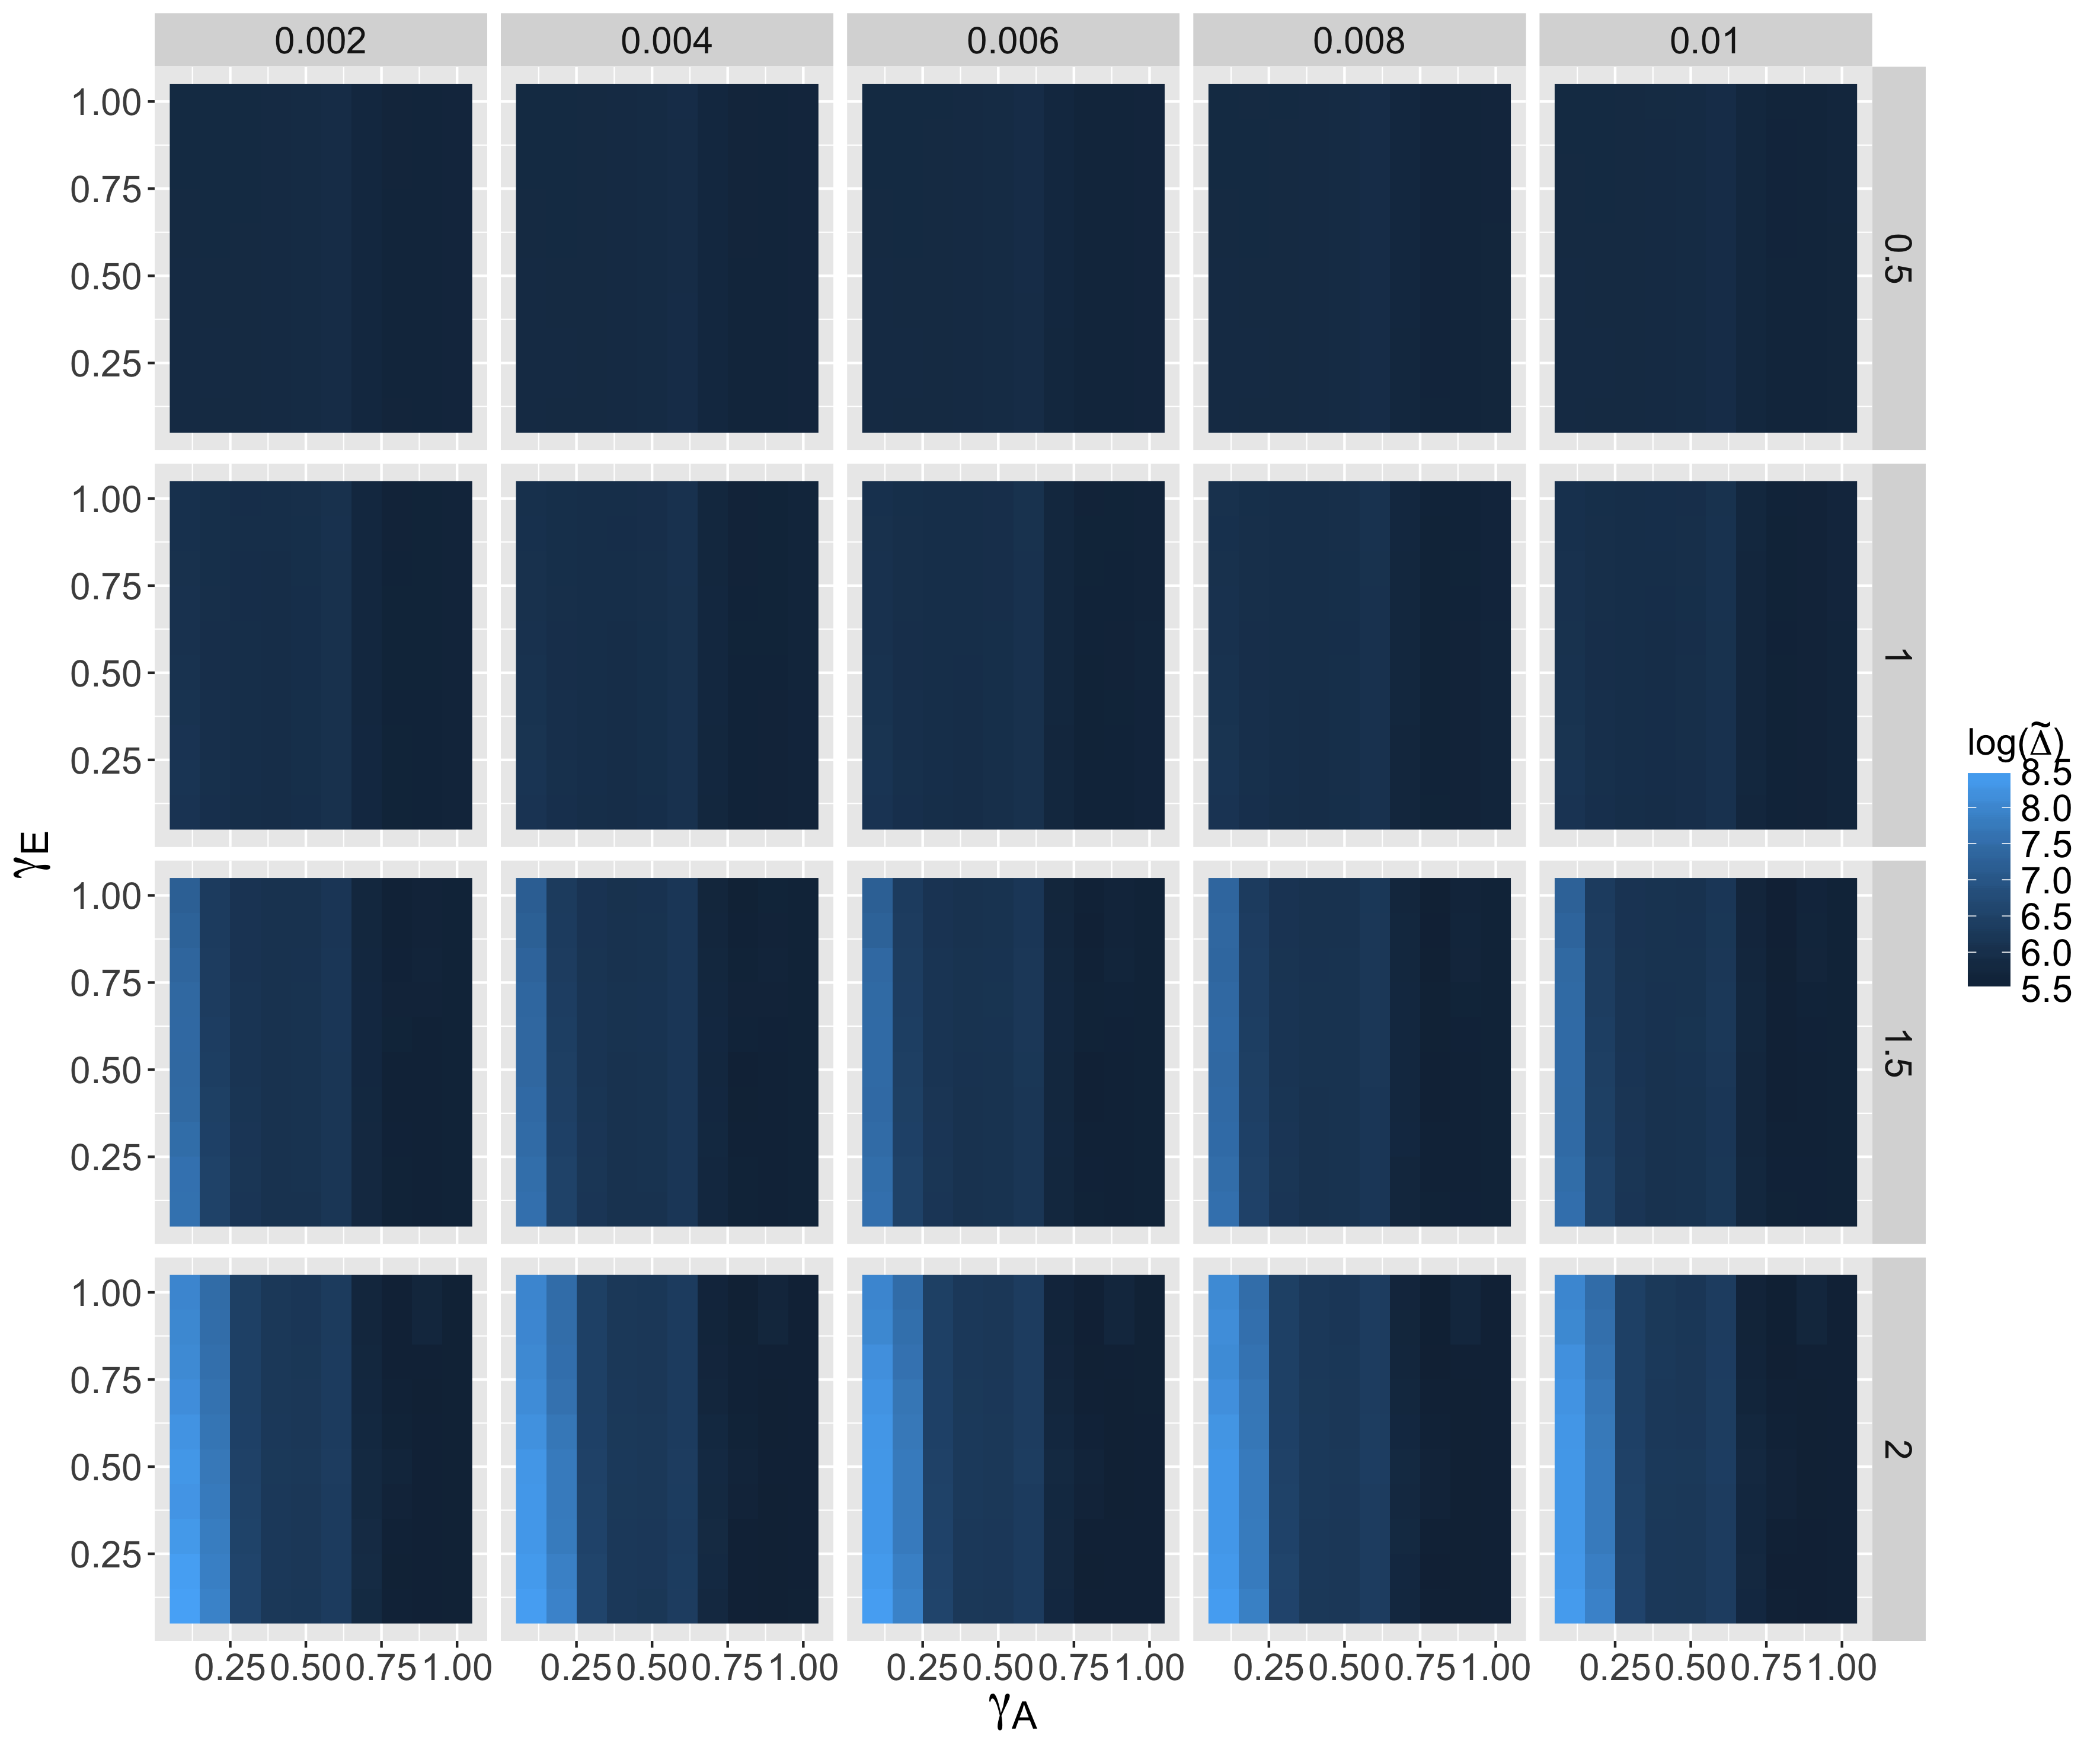
\includegraphics[width=\linewidth]{Figures/Lutecia/rdiffact_synth_nonw_euclpace6.png}
	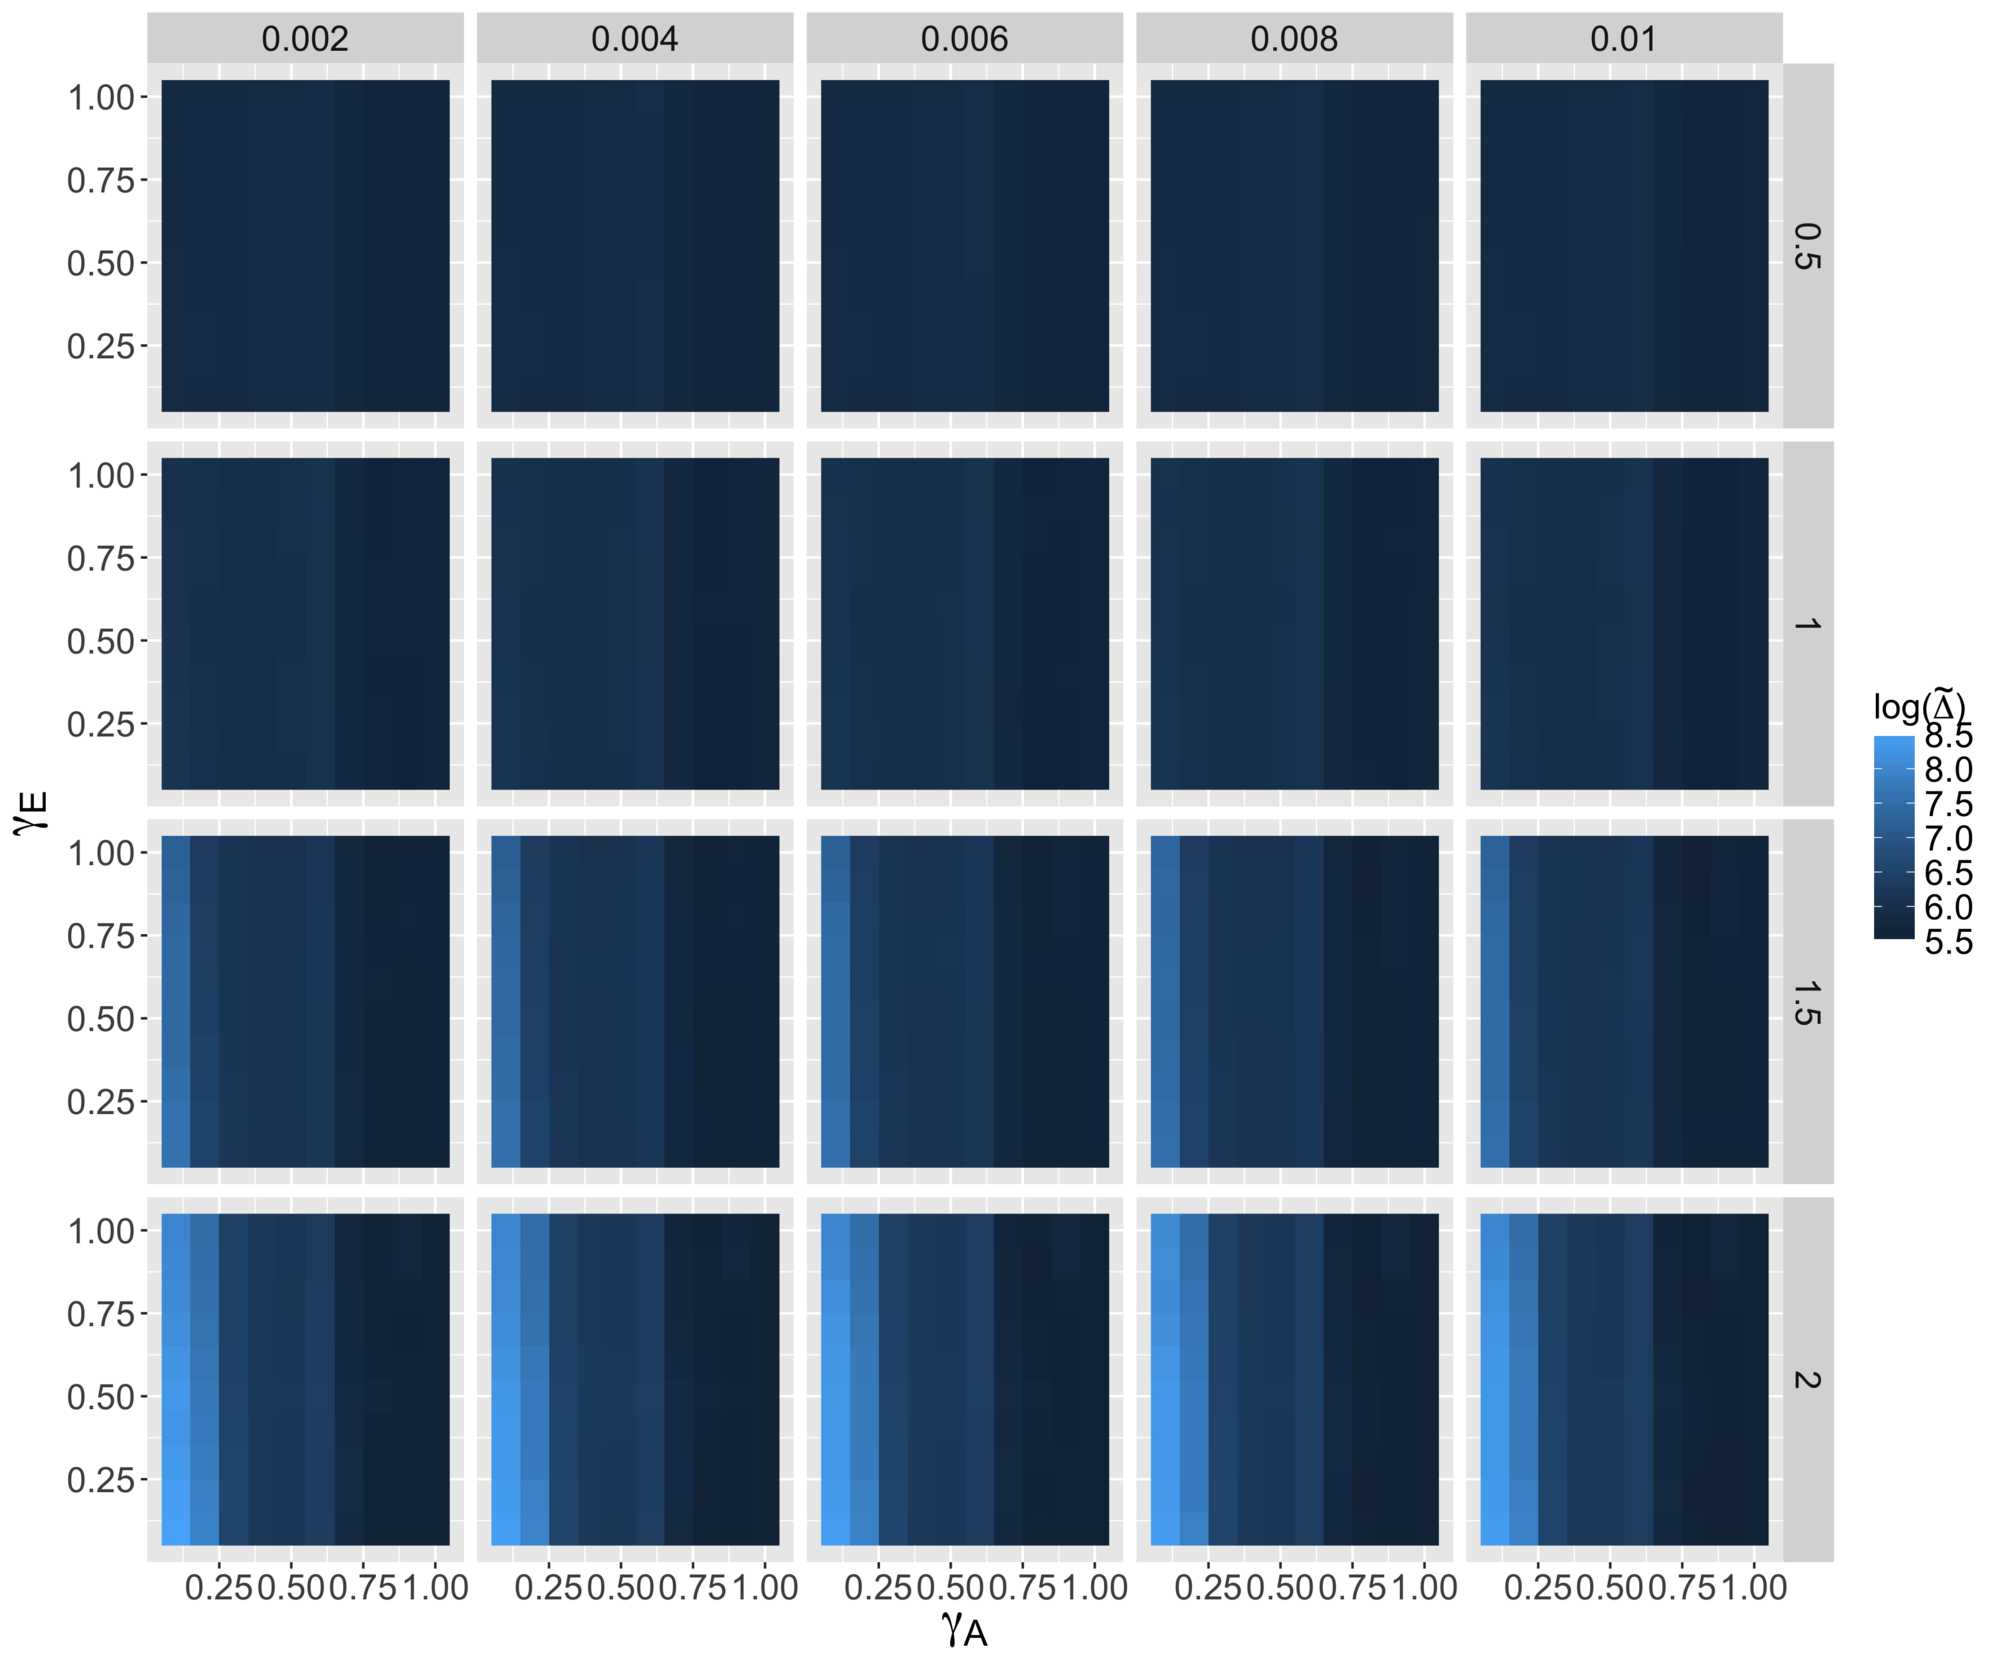
\includegraphics[width=\linewidth]{Figures/Final/A-lutecia-ludiff.jpg}
	\appcaption{\textbf{Cumulated variations of urban configurations.}\label{fig:app:lutecia:ludiff}}{\textbf{Variabilité cumulée des configurations urbaines.}\label{fig:app:lutecia:ludiff}}
\end{figure}
%%%%%%%%%%%%%%





%%%%%%%%%%%%%%%%%%%%%%%
\subsection{Transportation Sub-model}{Module de transport}

Nous n'avons pas pris en compte les flux de transport dans notre implémentation du modèle, supposant que les infrastructures construites sont de capacités suffisantes pour ne pas être significativement sensibles à la congestion.


Pour le calcul des flux entre cellules, l'opération est la suivante : les flux $\phi_{ij}$ sont calculés par résolution sur $p_i,q_j$ par une méthode de point fixe (algorithme de Furness), du système des flux gravitaires :


\[
\begin{cases}
\phi_{ij} = p_i q_j A_i E_j \exp{\left(-\lambda_{tr} d_{ij}\right)}\\
\sum_k \phi_{kj} = E_j\\
\sum_k \phi_{ik} = A_i\\
p_i = \frac{1}{\sum_k{q_k E_k \exp{(-\lambda_{tr}d_{ik})}}}\\
q_j = \frac{1}{\sum_k{p_k A_k \exp{(-\lambda_{tr}d_{kj})}}} 
\end{cases}
\]

où $\lambda_{tr}$ est un paramètre donnant la portée spatiale des flux journaliers.

Pour implémenter l'étape de distribution des flux dans le réseau, une fois les flux entre cellules connus, il faudrait par exemple déterminer les flux de l'Equilibre Utilisateur Statique avec un algorithme approprié. Une affectation par plus courts chemins est implémentée avec le calcul des flux dans le modèle, mais nous désactivons ce processus pour simplifier l'étude du modèle.


\bpar{
Trajectories are then attributed by effective shortest path, and corresponding congestion $c$ is computed on the corresponding flows (we do not complicate with a User Equilibrium or more complicated traffic assignment procedure). The speed of network given by BPR function $v(c) = v_0 \left(1 - \frac{c}{c_max}\right)^{\gamma_c}$. Congestion is not used in current studies (infinite capacity $\kappa$).
}{
La congestion peut être calculée comme un rapport à la capacité, comme $c/c_{max}$ si $c$ est le flux et $c_{max}$ la capacité. La vitesse est obtenue par une fonction BPR sous la forme $v(c) = v_0 \left(1 - \frac{c}{c_max}\right)^{\gamma_c}$. Notre configuration revient à supposer une capacité infinie  $c_{max} = \infty$.
}


\subsection{Cooperation probabilities}{Probabilités de coopération}


L'hypothèse d'équilibre implique que les espérances conditionnelles de chaque joueur sont égales étant donné leur deux choix, i.e. que 
\[
\Eb{U_i|S_i=C} = \Eb{U_i|S_i=NC}
\] 

Cela revient en effet dans ce cas à maximiser $\Eb{U_i}$ par rapport à $p_i$, puisque en conditionnant on a $\Eb{U_i} = p_i \Eb{U_i|S_i = C} + (1 - p_i) \Eb{U_i|S_i = NC}$, et donc $\frac{\partial \Eb{U_i}}{\partial p_i} = \Eb{U_i|S_i = C} - \Eb{U_i| S_i = NC}$.

On a alors

\[
\Eb{U_i|S_i=C} = p_{1-i} U_i(S_i=C,S_{1-i}=C) + (1- p_{1-i}) U_i (S_i=C,S_{1-i}=NC)
\]

et donc 

\begin{equation*}
\hspace{-1cm}
\begin{split}
	p_{1-i} & U_i(S_i=C,S_{1-i}=C) + (1- p_{1-i}) U_i (S_i=C,S_{1-i}=NC) \\
	& = p_{1-i} U_i(S_i=NC,S_{1-i}=C) + (1- p_{1-i}) U_i (S_i=NC,S_{1-i}=NC)
\end{split}
\end{equation*}

ce qui donne

\[
p_{1-i} = - \frac{U_i(C,NC) - U_i(NC,NC)}{\left(U_i(C,C) - U_i(NC,C)\right) - \left(U_i(C,NC) - U_i(NC,NC)\right)}
\]

En substituant les expressions des utilités à partir de la matrice de gain, on obtient l'expression de $p_i$ en fonction du coût de collaboration $J$ et de la différence des différentiels d'accessibilité.


\subsubsection{Discrete choice coordination}{Coordination par choix discrets}


Pour déterminer la probabilité de coopération dans le cas des choix discrets, il s'agit de résoudre $f(p_i) = 0$ avec
\[
f(x) = \frac{1}{1+\exp\left[-\beta_{DC}\frac{\Delta_i}{1 + \exp(-\beta_{DC}(x \Delta_{1-i} - J))} - J\right]} - x
\]
où nous avons noté $\Delta_i = \Delta X_{i}(Z^{\star}_{C}) - \Delta X_{\bar{i}}(Z^{\star}_{i})$.

On a immédiatement $f(0) > 0 $ et $f(1) < 0$ et $f$ est continue, il existe donc toujours une solution $x\in [0,1]$ par le théorème des valeurs intermédiaires.

Concernant l'unicité, il est possible de la montrer sous certaines conditions. Un calcul de $\frac{\partial f}{\partial x}$ donne 
\[
\frac{\partial f}{\partial x} = 2 (\cosh u(x) - 1) + \beta^2 \Delta_i \Delta_{1-i} \frac{\exp(-\beta_{DC}(x \Delta_{1-i} - J))}{(1 + \exp(-\beta_{DC}(x \Delta_{1-i} - J)))^2}
\]

où $u(x) = -\beta_{DC} (\frac{\Delta_i}{1 + \exp(-\beta_{DC}(x \Delta_{1-i} - J))} - J)$.

Comme $\cosh u \geq 1$, on a $\frac{\partial f}{\partial x} > 0$ si $\Delta_i \Delta_{1-i} > 0$. La fonction est dans ce cas strictement croissante et on a une unique solution.

En pratique, la solution est déterminée par algorithme de Brent, avec les bornes $[0,1]$ et une tolérance de $0.01$.


%%%%%%%%%%%%%%%%%%%%%%%
\subsection{Implementation details}{Détails d'implémentation}


\paragraph{Distance Matrix}{Matrice des distances}

\bpar{
Distance via network are updated in a dynamical programming fashion for efficiency purposes (because of the numerous network updates), the following way :
\begin{enumerate}
\item Euclidian distance matrix $d(i,j)$ is computed analytically
%\item Network shortest paths between network intersections (rasterized network) updated in a dynamic way (addition of new paths and update or change of old paths if needed when a link is added), correspondance between network patches and closest intersection also updated dynamically ; $O(N_{inters}^3)$
%\item Weak component clusters and distance between clusters updated ; $O(N_{nw}^2)$
%\item Network distances between network patches updated, through the heuristic of only minimal connexions between clusters ; $O(N_{nw}^2)$
%\item Effective distances (taking paces/congestion into account) updated as minimum between euclidian time and \[\min_{C,C'}{d(i,C)+d_{nw}(p_C(i),p_C'(j))+d(C',j)}\], complexity in $O(N_{clusters}^2\cdot N^2)$ (Approximated with $\min_C$ only in the implementation, consistent within the interaction ranges $\sim$ 5 patches taken in the model). 
\end{enumerate}
}{
La matrice des distances est mise à jour de manière dynamique pour des questions de rapidité d'execution (vu le nombre de mises à jour du réseau), de la façon suivante :
\begin{enumerate}
	\item La matrice de distance euclidienne $d(i,j)$ est calculée analytiquement
	\item Les plus courts chemins entre les intersections des liens (entre les cellules du réseau raster correspondant) sont mis à jour de manière dynamique (étape de complexité $O(N_{inters}^3$) :
	\begin{itemize}
		\item Pour chaque nouvelle intersection, les plus courts chemins vers l'ensemble des autres intersections sont calculés par l'ancienne matrice et le nouveau lien.
		\item Pour l'ensemble des anciens plus courts chemins, ils sont mis à jour si besoin après vérification des éventuels raccourcis par le nouveau lien.
		\item La correspondance entre les cellules quelconques du réseau et les intersections est mise à jour.
	\end{itemize}
	\item Les composantes connexes et les distances entre celles-ci sont mises à jour (complexité en $O(N_{nw}^2)$)
	\item Les distances par le réseau entre les cellules du réseau sont mises à jour, avec l'heuristique des connexions minimales uniquement (un lien unique le plus court entre chaque cluster) (complexité en $O(N_{nw}^2)$)
	\item Les distances effectives entre l'ensemble des cellules (prenant la vitesse et la congestion en compte si celle-ci est implémentée) sont calculées comme le minimum entre la distance euclidienne et 
	\[\min_{C,C'}{d(i,C)+d_{nw}(p_C(i),p_C'(j))+d(C',j)}\]
	dont nous prenons une approximation avec $\min_C$ uniquement dans l'implémentation, ce qui est consistant avec les portées d'interaction relativement faibles considérées. La complexité est en $O(N_{clusters}^2\cdot N^2)$.
\end{enumerate}
}


\paragraph{Network growth}{Croissance du réseau}


Les infrastructures potentielles, au nombre de $N_I$ lors de la recherche heuristique d'une infrastructure optimale, sont tirées aléatoirement parmi l'ensemble des infrastructures possibles ayant une extrémité au centre d'une cellule. Si l'extrémité est à une distance inférieure à un seuil $\theta_I$ d'un lien déjà existant du réseau, celle-ci est remplacée par sa projection sur le lien correspondant. Il s'agit de l'étape d'accrochage permettant d'obtenir un réseau de forme raisonnable localement. En cohérence avec la représentation raster du réseau, nous prenons $\theta_I = 1$, ce qui correspond à la taille d'une cellule. 






%%%%%%%%%%%%%%%%%%
\subsection{Setup}{Initialisation}


\subsubsection{Synthetic setup}{Initialisation synthétique}

\bpar{
This section describes the setup in the case of synthetic configurations of MCR.
}{
Nous décrivons ici les détails de l'initialisation synthétique.
}


\bpar{
Initial distribution of Actives and Employments is done around governance centers at positions $\vec{x}_i$ using exponential kernels by
}{
Les distributions initiales des actifs et des emplois dans la configuration synthétique sont pris autour des centres de gouvernance (maires) aux positions $\vec{x}_i$ avec des noyaux exponentiels par
}

\[
A(\vec{x}) = A_{max} \cdot \exp{\left(\frac{\norm{\vec{x}-\vec{x}_i}}{r_A}\right)} ; 
E(\vec{x}) = E_{max} \cdot \exp{\left(\frac{\norm{\vec{x}-\vec{x}_i}}{r_E}\right)}
\]



\subsubsection{Setup on a real configuration}{Initialisation sur configuration réelle}

Nous montrons en Fig.~\ref{fig:app:lutecia:realsetup} la population et les réseaux sur lesquels les expériences sur données réelles sont menées : à usage du sol fixe,
\begin{itemize}
	\item une expérience sans réseau initial, et avec pour réseau cible de calibration le réseau de 2010 ;
	\item une expérience avec le réseau initial de 2010, et pour réseau cible le réseau planifié.
\end{itemize} 


%%%%%%%%%%%%%
\begin{figure}
	%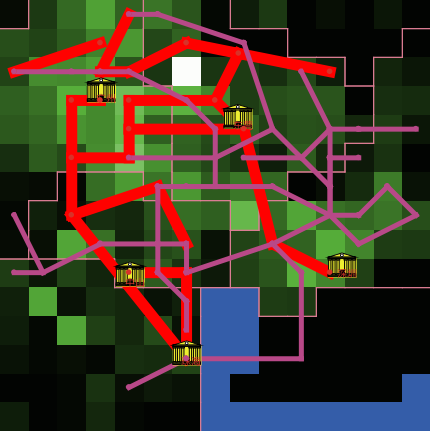
\includegraphics[width=\linewidth]{Figures/Lutecia/ex_real_filesetup.png}
	%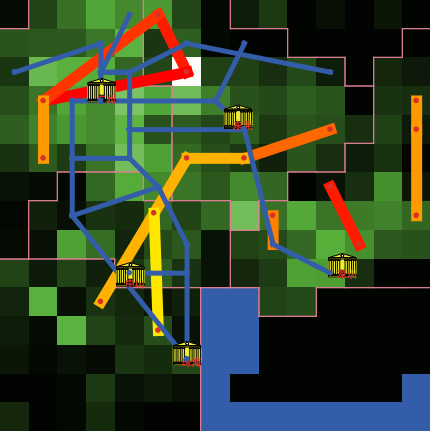
\includegraphics[width=\linewidth]{Figures/Lutecia/realnonw_nolu.png}
	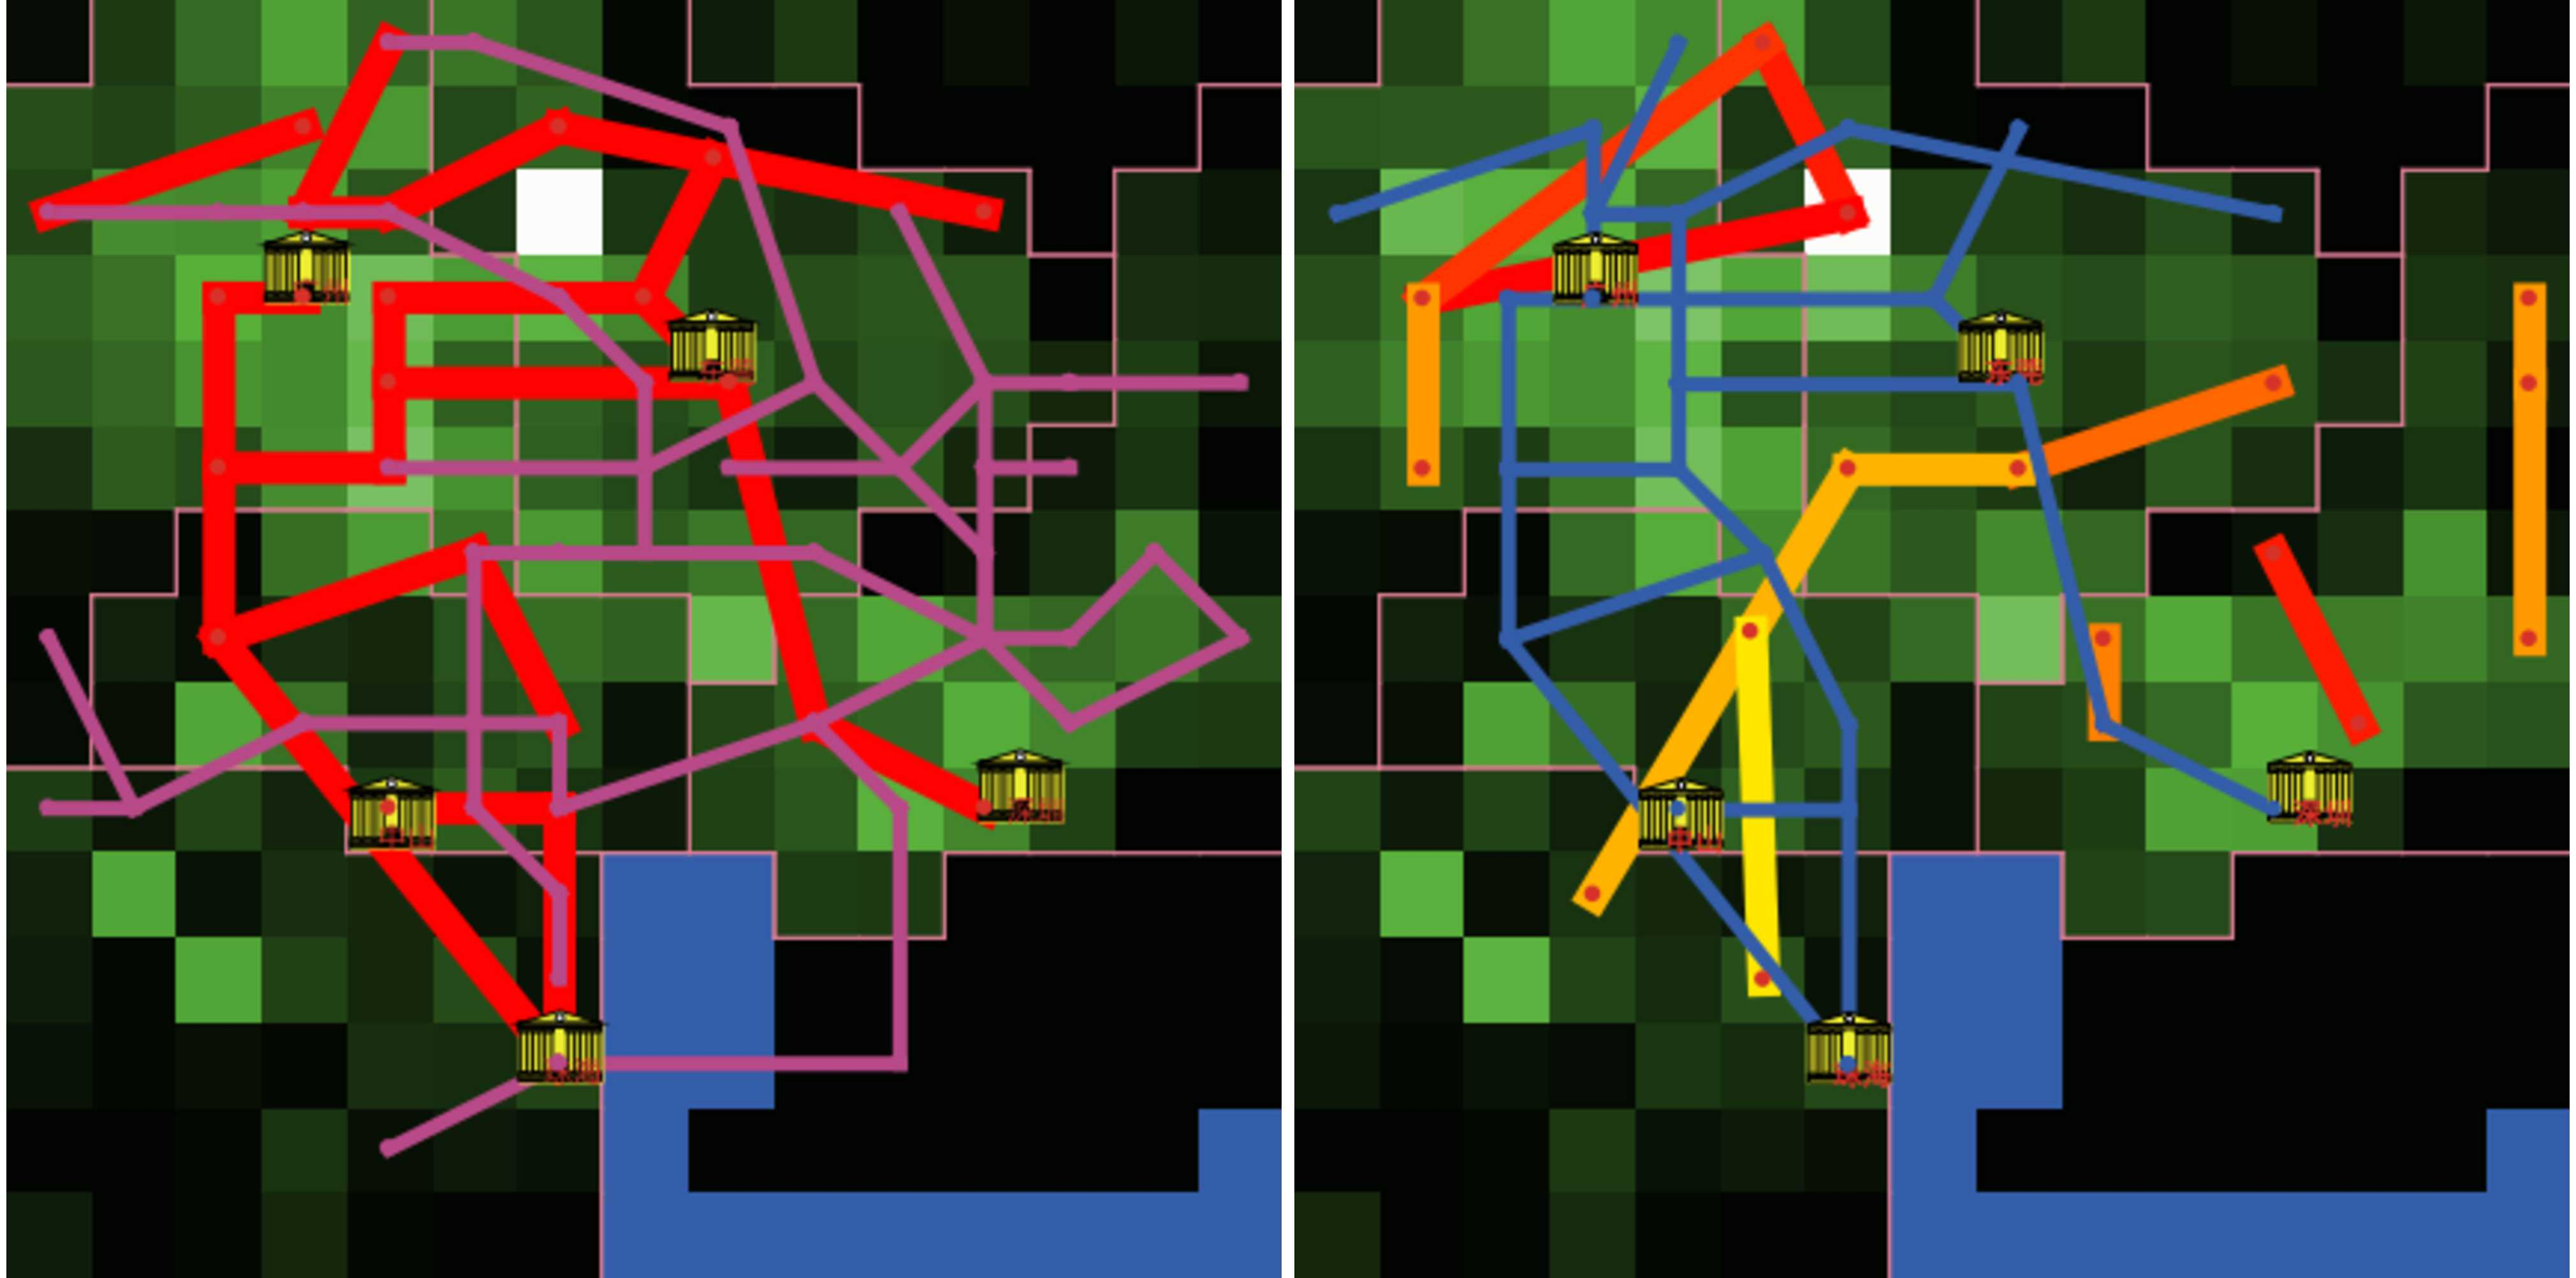
\includegraphics[width=\linewidth]{Figures/Final/A-lutecia-realsetup.jpg}
	\appcaption{\textbf{Setup on real data used for model application.}\label{fig:app:lutecia:realsetup}}{\textbf{Initialisation sur données réelles utilisée lors de l'application.} Pour des raisons de performances computationnelle, le nombre de cellules est ici diminué par rapport à l'illustration en texte principal. (\textit{Gauche}) Réseaux à l'initialisation, en rouge le réseau initial correspondant au réseau en 2010, en violet fin le réseau cible pour la calibration, correspondant au réseau planifié. (\textit{Droite}) Résultat obtenu avec $\alpha = 0$ à $t_f = 11$ après une initialisation sans réseau ; en bleu le réseau cible, qui correspond au réseau de 2010.\label{fig:app:lutecia:realsetup}}
\end{figure}
%%%%%%%%%%%%%

 









